\chapter{The closed loop}
\label{ch:closed}

\begin{figure}[h]
\centering
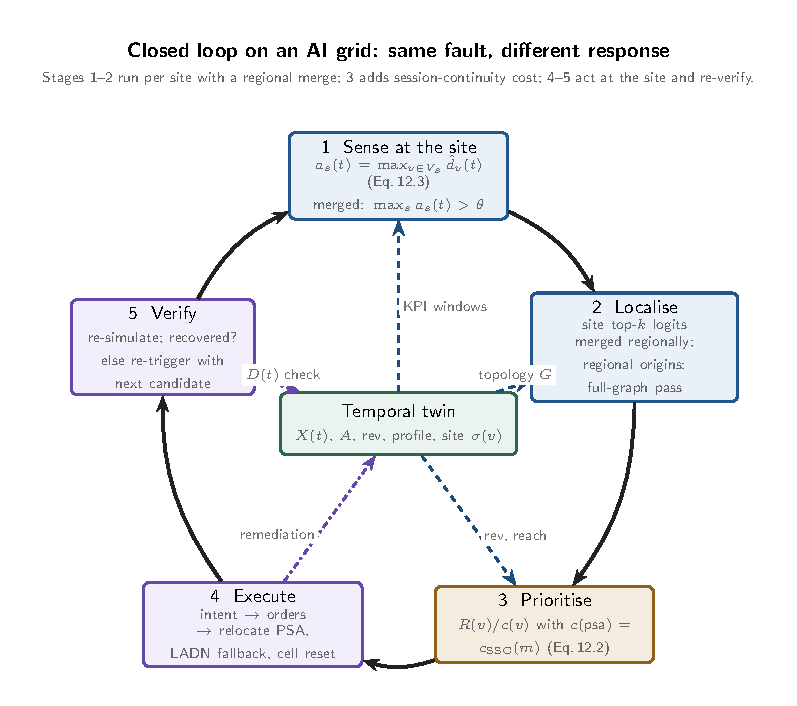
\includegraphics[width=0.78\textwidth]{../design/closed_loop.pdf}
\caption{Five stages around a twin. The only input is the KPI stream; the only output is an
ordered set of per-domain actions. Stages 1--2 are the learned model, stage 3 a one-line rule,
stages 4--5 plumbing and verification.}
\end{figure}

\section{Decomposition}
An intent with $n$ ordered targets decomposes into $n$ service orders, one per target, each
carrying the domain (RAN, Core, Transport), the target node and the remediation operation. In the
repository the intent is TMF921-shaped and the orders are TMF641-shaped: the field names follow
the standards so that a real orchestrator could be substituted for the mock, but we do not claim
conformance to either specification. The mock orchestrator records each order and returns the
step at which the highest-priority action takes effect.

\section{Measuring the loop}
The twin makes the loop measurable. We re-simulate the same fault with the injection removed from
the effective remediation step onward and record the recovery time, and we integrate the
revenue-weighted degradation over the episode:
\begin{equation}
\mathrm{Loss}=\sum_{t}\sum_{u\in\V}\mathrm{rev}_u\,d_u(t).
\label{eq:exposure}
\end{equation}
Comparing \eqref{eq:exposure} for a GNN-timed remediation against a threshold-timed one turns the
lead time of Chapter~\ref{ch:detection} into a business number on the same twin. If the model's
top-ranked origin is wrong, the remediation is applied to the wrong node, the injection is not
removed, and the GNN-timed loss is \emph{not} reduced; the metric therefore penalises wrong
root causes rather than rewarding confident ones.
